% ===================================================================
%  Week 5 — Lecture Notes (Persian) — Edge Detection
% ===================================================================
\documentclass[12pt,a4paper]{article}
% ===================================================================
%  Shared preamble for Persian lecture notes (Image Processing).
%  Compile with XeLaTeX.  Body = Persian (RTL), code/math = LTR.
% ===================================================================

\usepackage{geometry}
\geometry{a4paper,margin=2.4cm}
\usepackage{amsmath,amssymb}
\usepackage{graphicx}
\usepackage{xcolor}
\usepackage{listings}
\usepackage{tcolorbox}
\usepackage{booktabs}
\usepackage{array}
\usepackage{enumitem}
\usepackage{hyperref}
\tcbuselibrary{skins,breakable}

% ---- Persian / RTL --------------------------------------------------
\usepackage{xepersian}
\settextfont{IRNazli}
\setlatintextfont{Latin Modern Roman}
\setdigitfont{IRNazli}
% More generous leading + paragraph spacing (Persian reads better with air).
\linespread{1.5}
\setlength{\parskip}{0.7em}

% ---- Colours --------------------------------------------------------
\definecolor{coursePrimary}{HTML}{1B4965}
\definecolor{courseAccent}{HTML}{E76F51}
\definecolor{courseGood}{HTML}{2A9D8F}
\definecolor{courseBad}{HTML}{C0392B}
\definecolor{courseInfo}{HTML}{2980B9}
\definecolor{codeBg}{HTML}{F5F6FA}
\definecolor{codeKw}{HTML}{8E44AD}
\definecolor{codeStr}{HTML}{2A9D8F}
\definecolor{codeCom}{HTML}{7F8C8D}

\hypersetup{colorlinks=true,linkcolor=courseInfo,urlcolor=courseInfo,citecolor=courseInfo}

% ---- Code listings (Python built in) -------------------------------
\lstdefinestyle{course}{
  backgroundcolor=\color{codeBg},
  basicstyle=\ttfamily\small,
  keywordstyle=\color{codeKw}\bfseries,
  stringstyle=\color{codeStr},
  commentstyle=\color{codeCom}\itshape,
  numberstyle=\tiny\color{codeCom},
  numbers=left, numbersep=7pt,
  showstringspaces=false, breaklines=true,
  tabsize=4, columns=fullflexible, frame=single,
  rulecolor=\color{gray!30}, keepspaces=true, upquote=true, language=Python,
}
\lstset{style=course}
\lstdefinelanguage{bash}{
  keywords={cd,pip,python,venv,source,import}, sensitive=true,
  morecomment=[l]{\#}, morestring=[b]', morestring=[b]",
}
\newenvironment{ltrcode}{\begin{LTR}}{\end{LTR}}

% ---- Callout boxes (Persian titles) --------------------------------
\newtcolorbox{yaddasht}{colback=courseInfo!8,colframe=courseInfo,
  title={\textbf{یادداشت}},boxrule=0.6pt,right=6pt,left=6pt,breakable}
\newtcolorbox{nokte}{colback=courseAccent!10,colframe=courseAccent,
  title={\textbf{نکتهٔ کلیدی}},boxrule=0.6pt,right=6pt,left=6pt,breakable}
\newtcolorbox{hoshdar}{colback=courseBad!8,colframe=courseBad,
  title={\textbf{هشدار / دام}},boxrule=0.6pt,right=6pt,left=6pt,breakable}
\newtcolorbox{riyazi}{colback=coursePrimary!6,colframe=coursePrimary,
  title={\textbf{ریاضیات}},boxrule=0.6pt,right=6pt,left=6pt,breakable}
\newtcolorbox{tamrin}{colback=courseGood!8,colframe=courseGood,
  title={\textbf{تمرین}},boxrule=0.6pt,right=6pt,left=6pt,breakable}

% ---- Header helper --------------------------------------------------
\newcommand{\coursemeta}[2]{%
  \begin{center}
  {\large\textbf{پردازش تصویرِ کاربردی}}\\[2pt]
  {\color{coursePrimary}\rule{\linewidth}{1pt}}\\[4pt]
  {\Large\textbf{#1}}\\[3pt]
  {\small جزوهٔ درس — #2}
  \end{center}\vspace{4pt}
}


\begin{document}
\coursemeta{جلسهٔ ۵ — تشخیصِ لبه}{هفتهٔ پنجم}

{\small\itshape مکملِ اسلایدهای انگلیسیِ جلسهٔ ۵. تصاویر از دیتاستِ واقعیِ شما (کنتور و پلاک) تولید شده‌اند. هدف: یافتنِ لبه‌ها (تغییراتِ ناگهانیِ شدت) با گرادیان، تا رسیدن به تشخیص‌گرِ Canny.}

\vspace{0.5cm}
\tableofcontents
\vspace{1cm}

% ===================================================================
\section{چرا این جلسه}

لبه‌ها مرزِ اشیا (صفحه، کنتور، ارقام) را نشان می‌دهند. برای DocScan، یافتنِ مرزِ صفحه/کنتور با
لبه‌ها شروع می‌شود؛ خروجیِ این هفته وارد گامِ «یافتنِ صفحه» می‌شود. یک لبه جایی است که شدت
\emph{به‌سرعت} تغییر می‌کند — که با \textbf{گرادیان} (یک کرنلِ بالاگذر) پیدایش می‌کنیم.

\begin{nokte}
لبه‌ها فرکانس‌بالا هستند (جلسهٔ ۳). پس همان‌طور که هموارسازی یک عملیاتِ پایین‌گذر بود، تشخیصِ لبه
یک عملیاتِ بالاگذر است. کرنلی که تفاوتِ همسایه‌ها را می‌گیرد (نه میانگینشان را)، لبه را می‌یابد.
\end{nokte}

\subsection{انواعِ لبه}

همهٔ لبه‌ها یکسان نیستند. سه نوعِ اصلی: (۱) \textbf{پله‌ای} (\lr{step}) — تغییرِ ناگهانیِ ایده‌آل؛
(۲) \textbf{شیب‌دار} (\lr{ramp}) — تغییرِ تدریجی (در تصاویرِ واقعی به‌خاطرِ تاریِ لنز رایج‌تر است)؛
(۳) \textbf{سقفی/خطی} (\lr{roof/line}) — یک خطِ نازک (مثلِ یک سیم یا مرزِ باریک). گرادیان روی
لبه‌های پله‌ای و شیب‌دار خوب کار می‌کند؛ برای خطوطِ نازک، لاپلاسین یا آشکارسازهای خط بهترند.

\begin{yaddasht}
در عملِ واقعی، لبه‌ها هرگز پله‌ایِ کامل نیستند — تاریِ لنز، نمونه‌برداری، و نویز آن‌ها را به شیب
تبدیل می‌کنند. برای همین «مکانِ دقیقِ لبه» خودش یک تصمیم است: مرکزِ شیب؟ نقطهٔ بیشینهٔ گرادیان؟
Canny نقطهٔ بیشینهٔ گرادیان را انتخاب می‌کند.
\end{yaddasht}

% ===================================================================
\section{لبه چیست؟}

یک لبه = یک تغییرِ سریعِ شدت (تاریک به روشن یا برعکس). ریاضی: یک \textbf{گرادیانِ} بزرگ؛ مشتقِ
شدت آنجا زیاد است.

\begin{riyazi}
اندازهٔ گرادیان: $|\nabla f| = \sqrt{f_x^2 + f_y^2}$؛ جهت: $\theta=\operatorname{atan2}(f_y,f_x)$.
که $f_x$ و $f_y$ مشتقِ افقی و عمودیِ تصویرند.
\end{riyazi}

\subsection{مشتق‌ها به‌عنوانِ کرنل}

مشتقِ گسسته یک تفاضل است، پس با یک کرنل محاسبه می‌شود:
\[
\text{Sobel-x:}\ \begin{bmatrix}-1&0&1\\-2&0&2\\-1&0&1\end{bmatrix}
\qquad
\text{Sobel-y:}\ \begin{bmatrix}-1&-2&-1\\0&0&0\\1&2&1\end{bmatrix}
\]
هر کدام یک تفاوت را روی پیکسل حساب می‌کند. مجموعشان صفر است (ناحیهٔ تخت صفر می‌دهد، همان‌طور که یک
کرنلِ لبه باید). Sobel-x لبه‌های \emph{عمودی} را می‌یابد (چون تغییرِ افقی را می‌سنجد) و Sobel-y
لبه‌های افقی را.

% ===================================================================
\section{Sobel روی کنتورِ واقعی}

\begin{center}
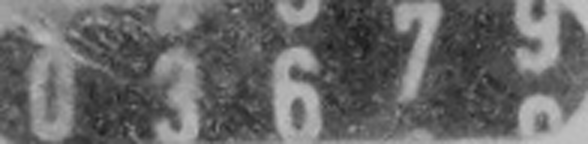
\includegraphics[width=0.9\linewidth]{../assets/meter_gray.png}\\[2pt]{\small تصویرِ خاکستری}\\[4pt]
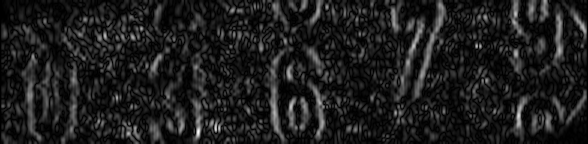
\includegraphics[width=0.44\linewidth]{../assets/meter_sobelx.png}\quad
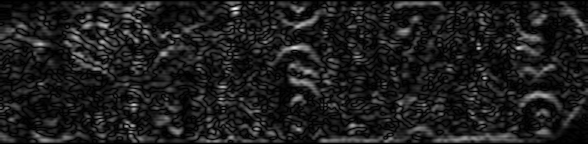
\includegraphics[width=0.44\linewidth]{../assets/meter_sobely.png}\\[2pt]
{\small چپ: گرادیانِ افقی ($\partial x$، لبه‌های عمودی) — راست: گرادیانِ عمودی ($\partial y$)}\\[4pt]
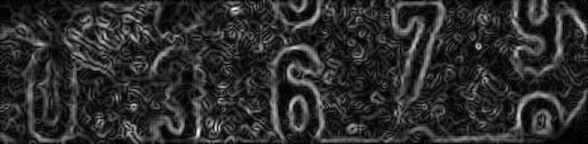
\includegraphics[width=0.9\linewidth]{../assets/meter_sobelmag.png}\\[2pt]{\small اندازهٔ گرادیان (ترکیبِ هر دو)}
\end{center}

\begin{itemize}
  \item \textbf{اندازه} $= \sqrt{g_x^2 + g_y^2}$: قدرتِ لبه (نقشهٔ لبهٔ روشن).
  \item \textbf{جهت} $= \operatorname{atan2}(g_y, g_x)$: لبه به کدام سو اشاره دارد (Canny از آن استفاده می‌کند).
\end{itemize}

\begin{hoshdar}
گرادیان‌ها به نویز حساس‌اند: نویز گرادیان‌های قویِ کاذب می‌سازد. همیشه اول هموار کنید (جلسهٔ ۳/۴).
مشتق‌گیری فرکانس‌بالا را تقویت می‌کند و نویز فرکانس‌بالاست — پس مشتقِ یک سیگنالِ نویزی توسطِ نویز
غالب می‌شود، نه لبه‌ها.
\end{hoshdar}

% ===================================================================
\section{ریاضیِ مشتقِ گسسته}

مشتقِ پیوستهٔ $\frac{df}{dx}$ در حالتِ گسسته با یک تفاضل تقریب زده می‌شود:

\begin{riyazi}
تفاضلِ مرکزی: $f_x(x) \approx \dfrac{f(x+1) - f(x-1)}{2}$ — که همان کرنلِ $[-1, 0, 1]$ (تقسیم بر ۲) است.
\end{riyazi}

Sobel یک گام جلوتر می‌رود: به‌جای یک ردیف، سه ردیف را با وزن‌های $[1, 2, 1]$ ترکیب می‌کند تا هم
مشتقِ افقی بگیرد و هم کمی در جهتِ عمودی هموار کند. برای همین Sobel از یک تفاضلِ سادهٔ $[-1,0,1]$
مقاوم‌تر به نویز است — هموارسازی و مشتق‌گیری را ترکیب کرده.

\begin{center}
\begin{tabular}{>{\raggedright\arraybackslash}p{0.35\linewidth} >{\raggedright\arraybackslash}p{0.55\linewidth}}
\toprule
\textbf{مشتقِ اول (گرادیان)} & \textbf{مشتقِ دوم (لاپلاسین)} \\
\midrule
لبه = بیشینهٔ مقدار & لبه = گذر از صفر \\
جهت‌دار (x و y جدا) & همه‌جهته (یک کرنل) \\
Sobel، Prewitt، Scharr & Laplacian، LoG \\
کمتر نویزی & بیشتر نویزی \\
\bottomrule
\end{tabular}
\end{center}

% ===================================================================
\section{مشتقِ دوم: لاپلاسین}

\[\text{Laplacian }= \begin{bmatrix}0&1&0\\1&-4&1\\0&1&0\end{bmatrix}\]

لبه‌ها را به‌صورتِ \textbf{گذر از صفر} (\lr{zero-crossing}) می‌یابد (جایی که مشتقِ دوم علامت عوض
می‌کند). یک کرنل، لبه‌ها را در همهٔ جهت‌ها می‌یابد — اما حتی به نویز حساس‌تر است.

\begin{center}
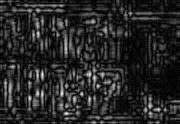
\includegraphics[width=0.5\linewidth]{../assets/plate_laplacian.png}\\[2pt]{\small لاپلاسینِ یک پلاک}
\end{center}

\textbf{LoG} (\lr{Laplacian of Gaussian}) اول هموار می‌کند، بعد لاپلاسین اعمال می‌کند — تا نویز
را رام کند. این ترکیبِ «اول هموار، بعد مشتق» موتیفِ کلِ این جلسه است.

% ===================================================================
\section{تشخیص‌گرِ Canny}

Canny یک کرنل نیست — یک الگوریتمِ ۴ مرحله‌ای است که لبه‌های تمیز، نازک و متصل تولید می‌کند:

\begin{enumerate}
  \item \textbf{هموارسازی} با گاوسی (حذفِ نویز).
  \item \textbf{گرادیانِ} اندازه و جهت (Sobel).
  \item \textbf{سرکوبِ غیربیشینه} (\lr{non-maximum suppression}): نازک‌کردنِ لبه‌های ضخیم به یال‌های تک‌پیکسلی.
  \item \textbf{آستانهٔ دوگانه + هیسترزیس}: نگه‌داشتنِ لبه‌های قوی، و لبه‌های ضعیفی که \emph{متصل} به قوی‌اند.
\end{enumerate}

\begin{center}
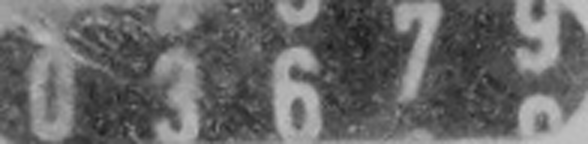
\includegraphics[width=0.9\linewidth]{../assets/meter_gray.png}\\[2pt]
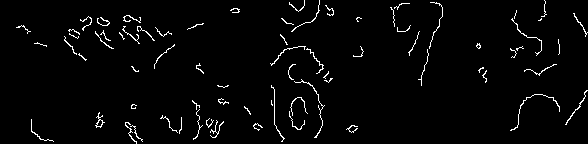
\includegraphics[width=0.9\linewidth]{../assets/meter_canny.png}\\[2pt]
{\small تصویرِ خاکستری (بالا) و لبه‌های Canny (پایین)}
\end{center}

\subsection{سرکوبِ غیربیشینه با جزئیات}

پس از محاسبهٔ گرادیان، لبه‌ها \emph{ضخیم}‌اند (چند پیکسل پهنا). \textbf{سرکوبِ غیربیشینه}
(\lr{NMS}) هر پیکسل را در \emph{جهتِ} گرادیانش با دو همسایه مقایسه می‌کند؛ اگر بیشینهٔ محلی نباشد،
صفر می‌شود. نتیجه: لبه‌های نازکِ تک‌پیکسلی. جهت به چهار حالت گِرد می‌شود (افقی، عمودی، دو قطر) تا
همسایه‌های درست انتخاب شوند.

مثال: اگر یک پیکسل روی یک لبهٔ عمودی است (گرادیان افقی)، با همسایه‌های \emph{چپ و راست}‌اش مقایسه
می‌شود؛ اگر از آن‌ها قوی‌تر نیست، حذف می‌شود. این تضمین می‌کند فقط «ستیغِ» لبه می‌ماند، نه دامنه‌هایش.

\begin{yaddasht}
NMS نمونهٔ دیگری از استفاده از \emph{جهتِ} گرادیان است (نه فقط اندازه). برای همین Canny هم اندازه و
هم جهت را محاسبه می‌کند. بدونِ NMS، لبه‌ها ضخیم و مبهم می‌مانند و یافتنِ کانتورِ دقیق (جلسهٔ ۹) سخت می‌شود.
\end{yaddasht}

\subsection{هیسترزیس: بخشِ هوشمندانه}

دو آستانه: \textbf{بالا} (قطعاً لبه) و \textbf{پایین} (شاید). هر لبهٔ قوی را نگه دارید، به‌علاوهٔ
لبه‌های ضعیفی که یک لبهٔ قوی را \emph{لمس} می‌کنند — و ضعیف‌های منزوی را دور بریزید. این شکاف‌ها را
روی یک لبهٔ واقعی پُر می‌کند در حالی که پاسخ‌های پراکندهٔ نویز را رد می‌کند.

\begin{ltrcode}
\begin{lstlisting}[language=Python]
blur  = cv2.GaussianBlur(gray, (5, 5), 0)     # step 1: smooth
edges = cv2.Canny(blur, 80, 160)              # low=80, high=160
# rule of thumb: high ~= 2-3x low
\end{lstlisting}
\end{ltrcode}

\begin{hoshdar}
حذفِ هموارسازی (یا آستانه‌های خیلی پایین) تصویر را با لبه‌های نویز پُر می‌کند. هیسترزیس دلیلِ آن
است که Canny کانتورهای بلند و متصل می‌دهد به‌جای یک آشوبِ لکه‌ای.
\end{hoshdar}

% ===================================================================
\section{مثالِ عددیِ Sobel}

بیایید Sobel-x را روی یک وصله حساب کنیم. فرض کنید یک لبهٔ عمودی داریم (چپ تاریک، راست روشن):
\[
P = \begin{bmatrix}10 & 10 & 200\\ 10 & 10 & 200\\ 10 & 10 & 200\end{bmatrix}
\qquad
K_x = \begin{bmatrix}-1 & 0 & 1\\ -2 & 0 & 2\\ -1 & 0 & 1\end{bmatrix}
\]
خروجیِ مرکز = مجموعِ ضربِ عنصربه‌عنصر:
\[
(-1)(10) + (0)(10) + (1)(200) + (-2)(10) + (0)(10) + (2)(200) + (-1)(10) + (0)(10) + (1)(200)
\]
\[
= -10 + 200 - 20 + 400 - 10 + 200 = 760
\]
یک مقدارِ بزرگِ مثبت — که نشان می‌دهد یک لبهٔ قوی با گذر از تاریک به روشن (از چپ به راست) وجود
دارد. اگر ستون‌ها برعکس بودند (روشن به تاریک)، مقدار منفیِ بزرگ می‌شد. پس \emph{علامتِ} گرادیان
جهتِ لبه را می‌گوید و \emph{اندازه‌اش} قدرتش را.

\begin{nokte}
حالا Sobel-x را روی یک ناحیهٔ تخت (همه ۱۰) امتحان کنید: هر جملهٔ مثبت با یک جملهٔ منفیِ متناظر
خنثی می‌شود و خروجی صفر است. برای همین گرادیان در نواحیِ تخت صفر و روی لبه‌ها بزرگ است — دقیقاً
آنچه می‌خواهیم.
\end{nokte}

% ===================================================================
\section{تمرینِ کلاسیِ وسط‌جلسه (۱۲ دقیقه)}

\begin{tamrin}
یک ردیفِ پیکسل: \lr{[10, 10, 10, 200, 200, 200]}. (۱) لبه کجاست؟ مشتقِ (اولِ) هر شکاف چیست
(تفاضل)؟ (۲) مشتق کجا \emph{بیشینه} است؟ آن را به «گرادیان = لبه» ربط دهید. (۳) اگر یک پیکسل نویز
باشد (\lr{[10,10,90,200,200,200]})، گرادیان چطور واکنش می‌دهد — و هموارسازی چطور کمک می‌کند؟
\end{tamrin}

\textbf{جمع‌بندی:} تفاضل‌ها: \lr{[0,0,190,0,0]} — مشتق در جهشِ $10\rightarrow200$ پیک می‌زند. آن
پیک \emph{همان} لبه است. بیشینهٔ مشتق = مکانِ لبه. آستانه‌گذاریِ مشتق، لبه‌ها را می‌یابد. پیکسلِ
نویز (۹۰) یک گرادیانِ کاذبِ کوچک‌تر می‌سازد؛ هموارسازی آن را میانگین می‌گیرد پیش از آنکه به یک لبهٔ
کاذب تبدیل شود.

% ===================================================================
\section{بخشِ عمیق}

\subsection{چرا پیش از مشتق‌گیری هموار کنیم}

مشتق‌گیری فرکانس‌بالا را \textbf{تقویت} می‌کند — از جمله نویز. پس مشتقِ یک سیگنالِ نویزی توسطِ نویز
غالب می‌شود، نه لبه‌ها. اول هموار کنید (گاوسی)، بعد مشتق بگیرید — پایهٔ Sobel/Canny/LoG.

\begin{riyazi}
اتحادِ کاربردی: (اول تار، بعد مشتق) = کانولوشن با \emph{مشتقِ گاوسی} — یک کرنل. یعنی می‌توان
هموارسازی و مشتق‌گیری را در یک کرنلِ واحد ادغام کرد.
\end{riyazi}

\subsection{خانوادهٔ عملگرها}

\begin{center}
\begin{tabular}{>{\raggedright\arraybackslash}p{0.2\linewidth} >{\raggedright\arraybackslash}p{0.35\linewidth} >{\raggedright\arraybackslash}p{0.35\linewidth}}
\toprule
\textbf{عملگر} & \textbf{ایده} & \textbf{نکته} \\
\midrule
\lr{Roberts} & تفاضلِ قطریِ $2\times2$ & کوچک، خیلی نویزی \\
\lr{Prewitt} & $3\times3$، وزنِ برابر & گرادیانِ ساده \\
\lr{Sobel} & $3\times3$، مرکز‌وزن & پیش‌فرضِ عملی \\
\lr{Scharr} & $3\times3$ بهینه & دقتِ چرخشیِ بهتر \\
\lr{Laplacian} & مشتقِ دوم & همهٔ جهت‌ها، یک کرنل \\
\bottomrule
\end{tabular}
\end{center}

همه یک مشتق را تخمین می‌زنند. Sobel/Scharr عملگرهای مرجعِ مشتقِ اول‌اند.

\subsection{کاربردهای تشخیصِ لبه}

لبه‌ها پایهٔ بسیاری از وظایفِ بینایی‌اند:

\begin{itemize}
  \item \textbf{یافتنِ شیء}: مرزِ صفحه، کنتور، پلاک (DocScan).
  \item \textbf{اندازه‌گیری}: طول/عرضِ یک قطعه از لبه‌هایش (بازرسیِ صنعتی).
  \item \textbf{تطبیق}: لبه‌ها ویژگی‌های پایدارتری از شدتِ خام‌اند (در برابرِ تغییرِ نور).
  \item \textbf{فشرده‌سازی/طرح}: بازنماییِ یک تصویر با لبه‌هایش.
  \item \textbf{بیناییِ رباتیک}: تشخیصِ راه، مانع، خطوط.
\end{itemize}

\subsection{کیفیتِ لبه: معیارها}

یک تشخیص‌گرِ لبهٔ خوب سه ویژگی دارد (معیارهای Canny): (۱) \textbf{تشخیصِ خوب} (لبه‌های واقعی را
بیابد، کاذب‌ها را نه)؛ (۲) \textbf{مکان‌یابیِ خوب} (لبه دقیقاً روی مرزِ واقعی باشد)؛ (۳)
\textbf{پاسخِ واحد} (هر لبه یک‌بار، نه چندین‌بار). خودِ الگوریتمِ Canny برای بهینه‌کردنِ همین سه
معیار طراحی شد — برای همین «استانداردِ طلایی» است.

\subsection{انتخابِ آستانه: auto-Canny}

آستانه‌های ثابت در نورهای مختلف شکست می‌خورند. آن‌ها را از میانهٔ تصویر مشتق کنید:
\lr{low = 0.66*median}، \lr{high = 1.33*median} — یک دستورِ شروعِ مقاوم. سپس روی تصاویرِ سخت
(کنتورِ سایه‌دار، کم‌کنتراست) تنظیم کنید.

\begin{ltrcode}
\begin{lstlisting}[language=Python]
def auto_canny(img, sigma=0.33):
    m = np.median(img)
    lo = int(max(0, (1.0 - sigma) * m))
    hi = int(min(255, (1.0 + sigma) * m))
    return cv2.Canny(img, lo, hi)
\end{lstlisting}
\end{ltrcode}

% ===================================================================
\section{تنظیمِ Canny در عمل}

اثرِ پارامترها را بفهمید تا بتوانید تنظیم کنید:

\begin{center}
\begin{tabular}{>{\raggedright\arraybackslash}p{0.35\linewidth} >{\raggedright\arraybackslash}p{0.55\linewidth}}
\toprule
\textbf{تغییر} & \textbf{اثر} \\
\midrule
آستانه‌ها را پایین بیاورید & لبه‌های بیشتر، شاملِ نویز \\
آستانه‌ها را بالا ببرید & فقط لبه‌های قوی؛ خطرِ از‌دست‌دادنِ لبه‌های ضعیف \\
هموارسازیِ بیشتر (پیش از Canny) & نویزِ کمتر، ولی لبه‌های ریز محو \\
نسبتِ high/low بزرگ‌تر & هیسترزیسِ سخت‌گیرتر (لبه‌های کمترِ متصل) \\
\bottomrule
\end{tabular}
\end{center}

\textbf{دستورِ عملی برای DocScan:} برای عکس‌های موبایلیِ کنتور، معمولاً یک هموارسازیِ گاوسیِ
$5\times5$ + auto-Canny (از میانه) نقطهٔ شروعِ خوبی است. سپس اگر مرزِ کنتور شکسته است، آستانهٔ
پایین را کم کنید؛ اگر لبه‌های نویز زیادند، هموارسازی یا آستانهٔ بالا را زیاد کنید. این تعادل را روی
سخت‌ترین عکس‌ها تنظیم کنید.

\begin{ltrcode}
\begin{lstlisting}[language=Python]
# a small experiment across thresholds
for lo, hi in [(30, 90), (80, 160), (120, 200)]:
    e = cv2.Canny(cv2.GaussianBlur(gray, (5, 5), 0), lo, hi)
    print(lo, hi, "-> edge pixels:", int((e > 0).sum()))
# pick the setting that gives a clean, connected boundary
\end{lstlisting}
\end{ltrcode}

\begin{nokte}
تعدادِ پیکسل‌های لبه یک سنجهٔ مفید است: خیلی زیاد یعنی نویز، خیلی کم یعنی از‌دست‌دادنِ ساختار.
اما بهترین سنجه، هدفِ نهایی است: آیا مرزِ صفحه/کنتور به‌طورِ کامل و متصل دیده می‌شود؟
\end{nokte}

% ===================================================================
\section{این جلسه در پروژهٔ نهایی}

\begin{itemize}
  \item Canny مرزِ صفحه/کنتور را به‌صورتِ لبه‌های متصل می‌دهد.
  \item بعدی (جلسهٔ ۹): از این لبه‌ها \textbf{کانتور} می‌یابیم و بزرگ‌ترین چهارضلعی را نگه می‌داریم — صفحه.
  \item سپس (جلسهٔ ۱۱): از ۴ گوشه‌اش برای تصحیحِ پرسپکتیو استفاده می‌کنیم. این هفته گامِ اول است.
\end{itemize}

\begin{nokte}
لبه‌ها هدف نیستند — مادهٔ خامِ یافتنِ \emph{شکل‌ها} (جلسهٔ ۹) و ساختارند. کیفیتِ لبه‌های امروز،
مستقیماً موفقیتِ یافتنِ صفحه در جلسهٔ ۹ را تعیین می‌کند.
\end{nokte}

\subsection{از لبه به خط: تبدیلِ هاف (Hough)}

گاهی لبه‌ها را به \emph{خط‌های} مستقیم می‌خواهید (مثلِ لبه‌های یک صفحهٔ مستطیلی). \textbf{تبدیلِ
هاف} (\lr{Hough transform}) هر نقطهٔ لبه را در یک فضای پارامتری (زاویه و فاصله) رأی می‌دهد؛
خط‌هایی که نقاطِ زیادی رویشان هستند، پیک‌های قوی می‌سازند. برای DocScan، هاف می‌تواند چهار لبهٔ
مستقیمِ صفحه را بیابد، حتی اگر Canny کمی شکسته باشد.

\begin{ltrcode}
\begin{lstlisting}[language=Python]
edges = cv2.Canny(gray, 80, 160)
lines = cv2.HoughLinesP(edges, 1, np.pi/180, threshold=80,
                        minLineLength=50, maxLineGap=10)
\end{lstlisting}
\end{ltrcode}

\begin{yaddasht}
تبدیلِ هاف نمونه‌ای از یک ایدهٔ قدرتمند است: \emph{رأی‌گیری}. هر شاهدِ محلی (یک نقطهٔ لبه) به همهٔ
ساختارهای سراسری‌ای که می‌تواند بخشی از آن‌ها باشد رأی می‌دهد، و ساختارهای واقعی رأی‌های زیادی
جمع می‌کنند. همین ایده در تطبیقِ ویژگیِ جلسهٔ ۱۰ (RANSAC) دوباره ظاهر می‌شود.
\end{yaddasht}

\subsection{لبه‌ها و یادگیریِ عمیق}

اولین لایهٔ یک CNN فیلترهای لبه/گرادیان را \emph{خودکار} می‌آموزد — اغلب شبیهِ Sobel. پس ویژگی‌هایی
که امروز دستی محاسبه می‌کنید، همان چیزی‌اند که یک شبکه خودش کشف می‌کند (جلسهٔ ۱۳). لبه‌های کلاسیک
همچنان مفیدند: سریع، قابلِ‌تفسیر، بدونِ نیاز به دادهٔ آموزشی.

% ===================================================================
\section{جمع‌بندی}

\begin{itemize}
  \item توضیحِ لبه به‌عنوانِ گرادیانِ بزرگ؛ محاسبهٔ Sobel-x/y، اندازه، جهت.
  \item استفاده از لاپلاسین/LoG؛ فهمِ گذر از صفر.
  \item اجرا و تنظیمِ تشخیص‌گرِ ۴ مرحله‌ایِ Canny؛ دانستنِ چراییِ هر گام.
  \item اتصالِ لبه‌ها به خطِ لولهٔ یافتنِ صفحهٔ DocScan.
\end{itemize}

\begin{tamrin}
\textbf{تحویلیِ این هفته (پیش از جلسهٔ ۶):} (۱) Sobel-x/y و اندازه را روی یک کنتور حساب و هرکدام
را نمایش دهید. (۲) Canny را اجرا کنید؛ اثرِ هموارسازی (با/بدون) و دو آستانه را نشان دهید. (۳)
auto-Canny را از میانه پیاده و با آستانه‌های دستی مقایسه کنید. (۴) DocScan: لبه‌های تمیزِ مرزِ
صفحه/کنتور را روی ۳ عکسِ واقعی به دست آورید.
\end{tamrin}

\subsection*{چک‌لیستِ دام‌های این هفته}

\begin{itemize}
  \item Canny بدونِ هموارسازیِ اول (سیلِ لبه‌های نویز) — همیشه اول تار کنید.
  \item آستانه‌های ثابت برای همهٔ تصاویر — از auto-Canny یا تنظیمِ per-image استفاده کنید.
  \item اعمالِ کرنلِ لبه روی \lr{uint8} (مقادیرِ منفی بریده می‌شوند) — به \lr{float} بروید.
  \item انتظارِ لبهٔ کامل و بسته — لبه‌ها اغلب شکسته‌اند؛ اتصال (هاف/مورفولوژی) لازم است.
  \item اشتباه‌گرفتنِ نقشهٔ گرادیان (ضخیم) با Canny (نازک/متصل).
\end{itemize}

\subsection*{واژه‌نامهٔ کوتاه}

\begin{center}
\begin{tabular}{>{\raggedright\arraybackslash}p{0.3\linewidth} >{\raggedright\arraybackslash}p{0.6\linewidth}}
\toprule
\textbf{اصطلاح} & \textbf{معنی} \\
\midrule
\lr{Edge} & تغییرِ سریعِ شدت (گرادیانِ بزرگ) \\
\lr{Gradient} & مشتقِ فضاییِ شدت (Sobel) \\
\lr{Laplacian / LoG} & مشتقِ دوم / لاپلاسینِ گاوسی \\
\lr{Canny} & الگوریتمِ ۴ مرحله‌ای لبه \\
\lr{Hysteresis} & آستانهٔ دوگانه برای اتصالِ لبه \\
\lr{NMS} & سرکوبِ غیربیشینه (نازک‌سازیِ لبه) \\
\bottomrule
\end{tabular}
\end{center}

\vspace{0.5cm}
\begin{center}
\textit{لبه جایی است که مشتق بزرگ است. هموار کن، مشتق بگیر، نازک کن، وصل کن — این Canny است.}
\end{center}

\end{document}
